\section{Durchführung}
\label{sec:Durchführung}
Zum experimentellen Aufbau gehört ein Ultraschall Doppler-Generator, eine Ultraschallsonde mit einer Frequenz von $\SI{2}{\mega\hertz}$ und ein Computer der mit der Sonde zur Datenaufnahme und -analyse verbunden ist.
Zusätzlich stehen Strömungsröhre mit verschiedenen Innen- und Außendurchmessern zur Untersuchung zur Verfügung.\\
Durch die Röhren strömt ein Gemisch aus Wasser, Glycerin und Glaskugeln.
Die Eigenschaften der Flüssigkeit wurden an die Frequenz der Ultraschallsonde angepasst.
Die Viskosität $\eta$ der Dopplerphantomflüssigkeit wird so verändert, dass sich bei einer mittleren Strömungsgeschwindigkeit eine laminare Strömung bildet.
Die Strömungsgeschwindigkeit wird mit einer Zentrifugalpumpe gesteuert.
Das Maß der Strömungsgeschwindigkeit ist die Umdrehungszahl der Pumpe $N$.\\
Die durch die Ultraschallsonde gemessenen Daten werden vom Computer erfasst und mit dem Programm FlowView verarbeitet.\\
Um mit der Sonde das Strömungsprofil zu messen wird ein Doppler-Prisma auf ein Rohr mit passendem Durchmesser gestellt.
Mit dem Ultraschallgel kann der Übergang zwischen Sonde zum Doppler-Prisma und Doppler-Prisma zum Rohr geschlossen werden.\\
\begin{wrapfigure}{r}{0.5\linewidth}
    \centering
    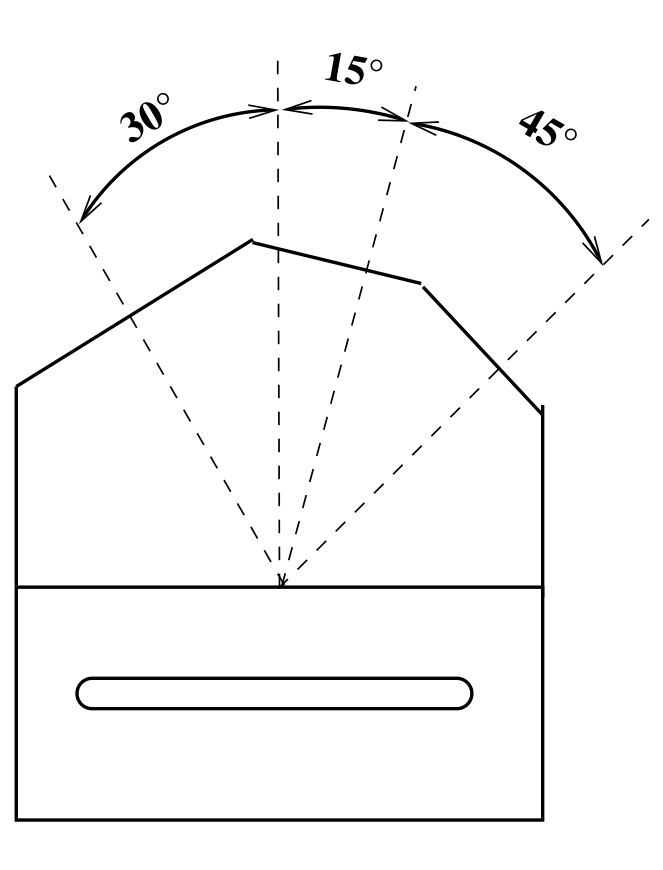
\includegraphics[width=0.75\linewidth]{content/data/doppler_prisma.jpg}
    \caption{Eine schematische Darstellung des Doppler-Prisma. \cite[3]{anleitung}}
    \label{fig:doppler_prisma}
\end{wrapfigure}
Das Doppler-Prisma ist in Abb. \ref{fig:doppler_prisma} skizziert.
Das Prisma besitzt drei Einstellwinkel $\theta$ mit gleichem Abstand zwischen Sonde und Rohr.
Der Dopplerwinkel ergibt sich aus dem Brechungsgesetz
\begin{equation}
    \alpha = \SI{90}{\degree} - \arcsin \left( \sin \theta \cdot \frac{c_L}{c_P} \right)
    \label{eqn:dopplerwinkel}
\end{equation}
, wobei $c_L$ die Schallgeschwindigkeit der Doppler-Flüssigkeit und $c_P$ die des Prismamaterials (hier Acryl) ist.
\\
\\
Zuerst soll die maximale Frequenz $f_\text{max}$ in Abhängigkeit der Strömungsgeschwindigkeit $N$ bestimmt werden.
Bei Geschwindigkeitsmessungen muss bei dem Ultraschallgenerator das SAMPLE VOLUME auf LARGE stehen.
Die Strömungsgeschwindigkeit wird an der Zentrifugalpumpe auf einen Wert festgelegt und dann dreimal die Frequenzverschiebung $\Delta \nu$ mit der Ultraschallsonde durch alle drei Dopplerwinkel gemessen.
Die Messung wird für fünf unterschiedliche Strömungsgeschwindigkeiten durchgeführt.
Aus der Verschiebung kann die Strömungsgeschwindigkeit bestimmt werden.
\\
\\
Im Anschluss soll das Strömungsprofil der Dopplerflüssigkeit an einem 3/8 Zoll -Schlauch mit dem Dopplerwinkel $\theta = \SI{15}{\degree}$ untersucht werden.
Hier ist es notwendig am Ultraschallgenerator das SAMPLE VOLUME auf SMALL zu stellen, damit die Messtiefe varriert werden kann.
Diese kann nun mit dem Regler DEPTH eingestellt werden.
Die Messtiefe ist in $\si{\micro\second}$ angegeben und für Acryl entsprechen $\SI{4}{\micro\second} = \SI{6}{\milli\metre}$.\\
Zunächst wird die Pumpleistung auf $\SI{70}{\percent}$ bzw. $N = \SI{6000}{\frac{1}{\minute}}$ eingestellt und die Strömungsgeschwindigkeit und den Streuintensitätswert gemessen.
Die Messtiefe $D$ wird im Intervall $\SI{12.5}{\micro\second} \leq D \leq \SI{19.0}{\micro\second}$ in $\Delta D = \SI{0.5}{\micro\second}$-Schritten variiert.\\
Die Messung wird für eine Pumpleistung von $\SI{45}{\percent}$ bzw. $N = \SI{3880}{\frac{1}{\minute}}$ wiederholt.